\documentclass[tikz]{standalone}
\usepackage{tikz}
\usepackage{tkz-euclide}
\usepackage{fourier-otf}
\usepackage{fontspec}

\usetikzlibrary{calc}

\begin{document}
	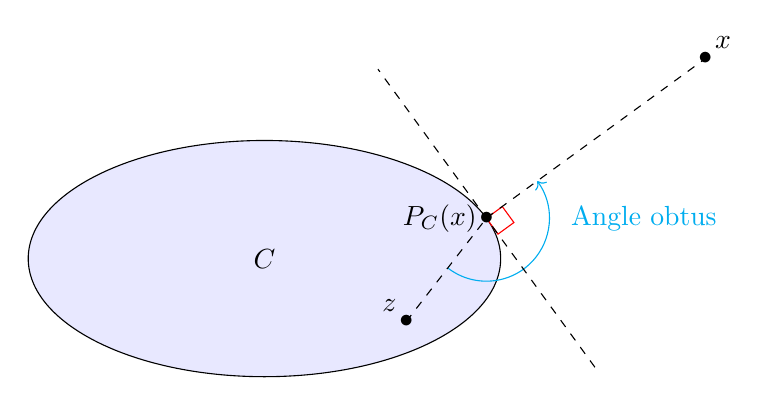
\begin{tikzpicture}
		\def\a{3}
		\def\b{1.5}
		\def\angle{20}
		
		\coordinate (O) at (0, 0);
		\coordinate (X) at (5.6, 2.54);
		\coordinate (Z) at (1.8, -0.8);
		\coordinate (P) at (\angle:{\a} and {\b});
		\coordinate (F1) at ({-sqrt(\a*\a-\b*\b)}, 0);
		\coordinate (F2) at ({+sqrt(\a*\a-\b*\b)}, 0);
		\tkzDefLine[bisector out](F1,P,F2) \tkzGetPoint{K}
		\coordinate (A) at ($(K)!+0.5!(P)$);
		\coordinate (B) at ($(P)!-0.5!(K)$);
		
		\draw[fill=blue!30, fill opacity=0.3] (O) ellipse ({\a} and {\b});
		
		\tkzMarkRightAngle[color=red](X,P,K);
		\tkzMarkAngle[->,size=0.8,color=cyan,mark=none](Z,P,X);
		\tkzLabelAngle[pos=0,shift={(2,0)}](Z,P,X){\color{cyan} Angle obtus};
		
		\draw(O) node {$C$};
		\draw(P) node{$\bullet$} node[left]{$P_C(x)$};
		\draw(X) node{$\bullet$} node[above right]{$x$};
		\draw(Z) node{$\bullet$} node[above left]{$z$};
		
		\draw[dashed] (A) -- (B);
		\draw[dashed] ($(A)!(X)!(B)$) -- (X);
		\draw[dashed] (Z) -- (P);
	\end{tikzpicture}
\end{document}